\section{Diseño}

El escenario se compone de tres entidades (ver figura \ref{fig:escenario}):
\begin{itemize}
 \item Service Provider.
 \item Service Provider 2.
 \item Identity Provider.
\end{itemize}

\begin{figure}[h!]
\centering
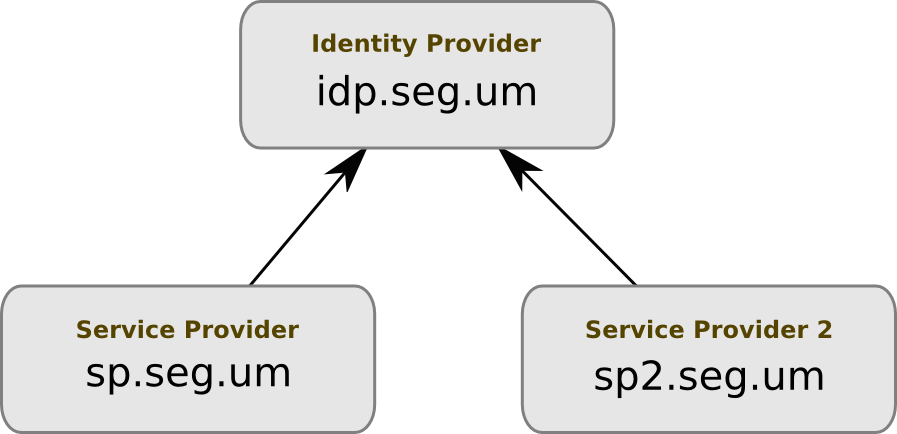
\includegraphics[width=0.7\textwidth]{img/escenario}
\caption{Escenario de la práctica y relaciones de confianza.}
\label{fig:escenario}
\end{figure}

Cada una de las máquinas ha sido montada en una máquina virtual con VirtualBox (ver figura \ref{fig:vbox}). Es requisito indispensable que los nombres de dominio indicados en la figura \ref{fig:escenario} sean resolubles en el cliente. Por ejemplo, configurándolos en el fichero \emph{/etc/hosts} en linux.

El entorno de ejecución es un contenedor Apache Tomcat, utilizando la tecnología Java EE para cada sitio. Un servlet es el encargado de recibir las peticiones y realizar la lógica del sitio.

Las redirecciones en todas las entidades se realizan con un POST.

\begin{figure}[h!]
\centering
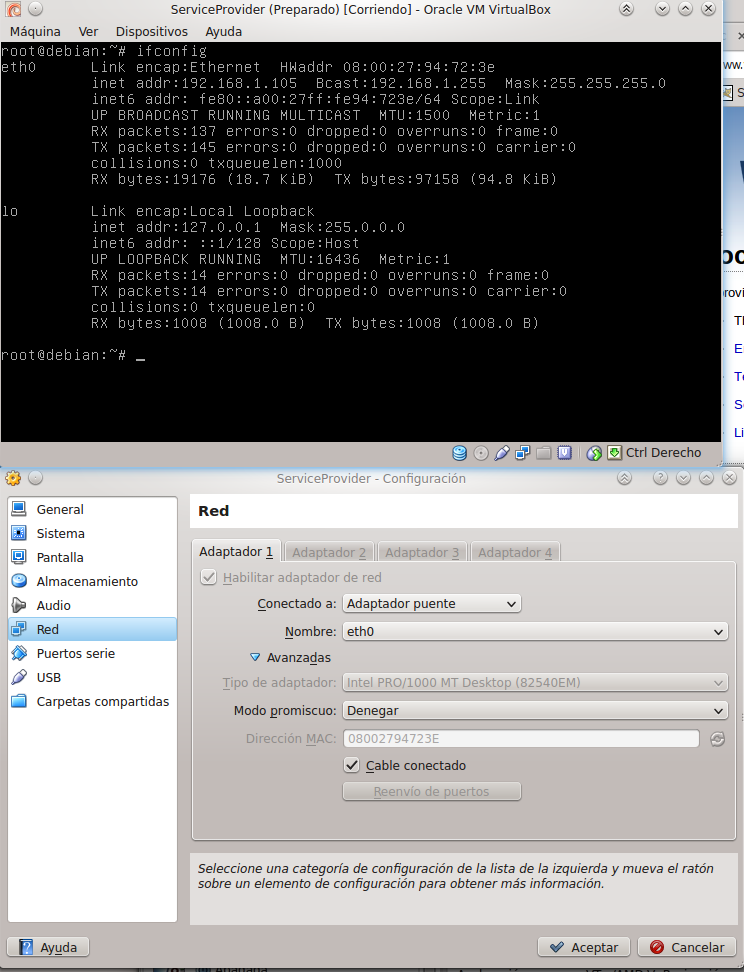
\includegraphics[width=0.7\textwidth]{img/maquinavirtual}
\caption{Maquina virtual ejecutandose en modo bridge.}
\label{fig:vbox}
\end{figure}